\documentclass[12pt,a4paper,titlepage]{report}

\usepackage{tcolorbox} % load the tcolorbox package (which loads the fancyvrb package)
\usepackage{minted}
% set up the minted package
\usemintedstyle{borland} % set the code highlighting style
\setminted{fontsize=\small} % set the code font size
\usepackage[backend=biber]{biblatex}
\addbibresource{references.bib}
\usepackage{graphicx}
\usepackage{subfig}
\usepackage{float}
\usepackage{tcolorbox}
\usepackage{parskip}
\usepackage{microtype}
\usepackage{fvextra}
\usepackage[margin=2cm]{geometry}
\usepackage{fancyhdr}
\usepackage{xcolor}
\usepackage{caption}

\let\cleardoublepage\clearpage

% Referencing
%
%
\addbibresource{references.bib}

% Graphics and colour
%

\usepackage{graphicx}
\graphicspath{{./diagrams/}}
\usepackage{xcolor} 
\usepackage{tcolorbox}

\definecolor{myOrange}{RGB}{241,85,44}
\definecolor{myGray}{RGB}{106,100,100}

% Page setup
%
\usepackage{fancyhdr}
\pagestyle{fancy}
\fancyhead{}
\fancyfoot{}
\renewcommand{\headrulewidth}{0.4pt}
\setlength{\headheight}{15pt}

\lhead{\rmfamily \textcolor{gray}{\AcademicTitle}}
\rhead{\rmfamily \textcolor{gray}{\Report}}
\lfoot{\rmfamily \textcolor{gray}{\Author (\StudentID)}}
\rfoot{\rmfamily \thepage}

\usepackage{parskip}
\usepackage[bottom]{footmisc}
% Document Info
%
\newcommand\AcademicTitle{Frankenstein Test-Suite Re-Architecture}
\newcommand\CommericalTitle{Bosco}
\newcommand\Author{Margaret McCarthy}
\newcommand\StudentID{20095610}

\newcommand\Date{March 2023}
\newcommand\Report{Project Report}
\newcommand\Stakeholder{ServisBOT Ltd.}
\newcommand\Course{Higher Diploma in Computer Science}
\newcommand\Reader{Supervisor: David Power}
\newcommand\University{South East Technological University}

\begin{document}

\pagenumbering{roman}

% title page 
\thispagestyle{empty}
\begin{center}
 \mbox{}\vfill
 {\fontsize{17pt}{20pt}\selectfont \bfseries \AcademicTitle}
 \vfill
 {\fontsize{14pt}{20pt}\selectfont \bfseries\itshape \CommericalTitle}
 \vfill
 {\fontsize{12pt}{20pt}\selectfont \bfseries \Report}
 \vfill
 {\fontsize{14pt}{20pt}\selectfont \bfseries \Author}
 \vfill
 {\fontsize{14pt}{20pt}\selectfont \bfseries \Stakeholder}
 \vfill
 {\fontsize{14pt}{20pt}\selectfont \bfseries \StudentID}
 \vfill
 {\fontsize{14pt}{20pt}\selectfont \bfseries \Reader}
 \vfill
 {\fontsize{14pt}{20pt}\selectfont \bfseries \Course}
 \vfill
 {\fontsize{14pt}{20pt}\selectfont \bfseries \University}
 \vfill
\end{center}
\clearpage

\tableofcontents

\listoftables

\listoffigures

% start of main matter
\clearpage
\pagenumbering{arabic}
\setcounter{page}{1}

\chapter{Introduction}

\section{Background}

This project aims to design and implement a feature based test runner for ServisBOT which determines which features of a system are working and which are down. The proposed system has the working title Bosco.

ServisBOT Ltd runs an online platform that creates chatbots which provide customer service by allowing end users to communicate with a business or service through a pop up messenger on a website. The technology is cloud based and mostly serverless which means it is provided over the internet rather than using storage on a physical computer or server. It has to be consistently monitored and so tests are run continuously to ensure any problems are detected and resolved immediately. Testing the code is crucial to the service they provide. It ensures a robust platform and gives customers confidence that the system is dependable.

\subsection{Frankenstein}
The components of a chatbot and each of its functions are broken down into micro services. These are created independent of one another but combined are the building blocks for the chatbot. There is a suite of tests which ServisBOT have called Frankenstein tests which run against these micro services. They run several times an hour, every hour. 
\subsection{TestCafe}
The tests use a software package called Testcafe which is an end to end testing service that uses messenger in a browser in order to run their tests. It simulates what a user would do by opening a browser and interacting with a chatbot. If the chatbot reacts in the expected way the test passes, otherwise the issue is investigated and resolved.
\subsection{EC2}
The Frankenstein test suite is run on two EC2 instances in two different AWS regions. AWS Elastic Compute Cloud (EC2) is basically a virtual machine where developers can define the resources they need. For example, what regions the are to be run in. 
\section{The Issue}

Running the tests causes a lot of contention for CPU and memory. When a test run is instigated all tests are competing for CPU usage because each EC2 instance is running thirty plus tests on one server which has limited memory.

Also there are numerous problems with Testcafe. 
\begin{itemize}
 \item Testcafe has proven to be resource heavy, expensive and inefficient, causing slow CPU performance. 
 \item Because of the competing resources some tests affect the performance of others. 
 \item Debugging and monitoring of the tests is complex.
 \item The test suite does not scale. Scalability is essential in order to increase the number of tests according to the number of user interactions and alternatively to reduce the number of tests when interactions drop which would not only prove to be more cost effective but would mostly solve all the issues mentioned.
\end{itemize}

 \begin{figure}[ht]
  \centering
  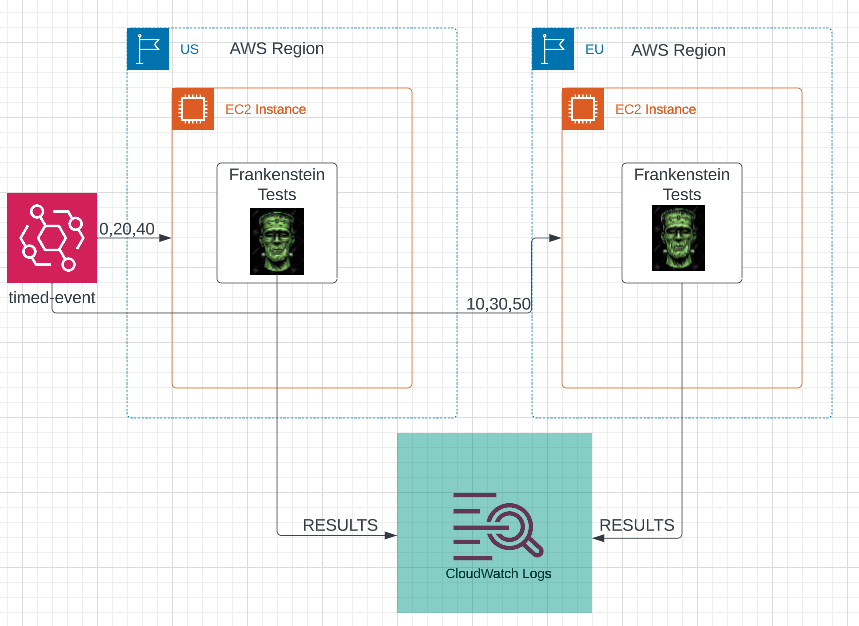
\includegraphics[width=\textwidth,height=\textheight,keepaspectratio]{./diagrams/frank_high_level.png}
  \caption{High level view of Frankenstein}
 \end{figure}
 \clearpage

\section{Purpose and Requirements for Bosco}

This project aims to completely overhaul the existing test suite by migrating the tests from the EC2 instances to AWS Lambda functions. This would ensure each lambda, whether it runs one test or multiple tests, is run independently and is not competing for memory. It would mean the test suite could be scaled infinitely, would run faster and as a result would most likely be a lot more cost efficient. This has yet to be proven.

In particular the migration will focus on an automation tool called Puppeteer which has been proven by ServisBOT to be more performant than Testcafe. The Puppeteer package includes its own browser whereas Testcafe launches an external browser which is slow and cumbersome. With Puppeteer there is more control over what the developer can test, it is more efficient, easier to debug and has a lot more functionality. It is widely chosen by developers now.

\begin{figure}[ht]
 \centering
 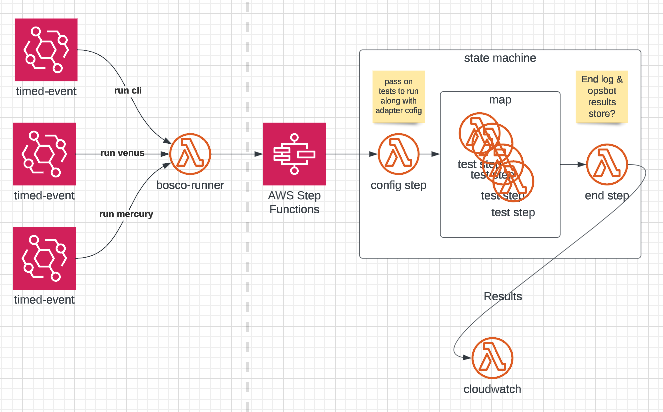
\includegraphics[width=\textwidth,height=\textheight,keepaspectratio]{./diagrams/bosco_high_level.png}
 \caption{High level view of Bosco}
\end{figure}

\chapter{Research and Development}

In order to determine the best approach, technologies and methodology for Bosco, it was concluded that the research and analysis phase necessary for the implementation of this project was the following:

\begin{itemize}
 \item Review of Frankenstein and Testcafe
 \item Cost Analysis of Frankenstein
 \item Research into possible testing frameworks for Bosco
 \item Puppeteer comparison to Testcafe
 \item Lambda vs EC2 comparison
 \item Possible implementations and modelling of Bosco
 \item Proof of Concept
 \item Additional requirements for implementing Bosco
 \item Scope of the project
\end{itemize}

\section{Review of Frankenstein and Testcafe}
Frankenstein is a feature based test runner designed to determine
which features of a system are up and working and which are down.
The tests are run in AWS ECS and are run on a cron.

\begin{table}[H]
 \centering
 \small
 \setlength\tabcolsep{6pt}
 \begin{tabular}{|c|c|}
  \hline \textbf
  {Pros} & \textbf {Cons}\\
  \hline\hline
  Cross Browser Testing&Expensive\\
  \hline
  Open Source& Slow\\
  \hline
  Easy Setup \& Installation& Difficult to debug\\
  \hline
  Built-In Waits& No browser control\\
  \hline
  Supports devices without extra software package & Simulated events leads to false positives\\
  \hline
  UI End to End Testing\\
  \hline
  Both client and server side debug \\
  \hline
 \end{tabular}
 \caption{Pros and Cons of Testcafe}
\end{table}

\section{Cost Analysis of Frankenstein Tests}

The following cost analysis was carried out on Frankenstein. There is an EC2 instance running the tests in the EU and the US costing ServisBOT about \$20 per day each. This costs the company almost \$15,000 a year to run tests.

\begin{figure}[ht]
 \centering
 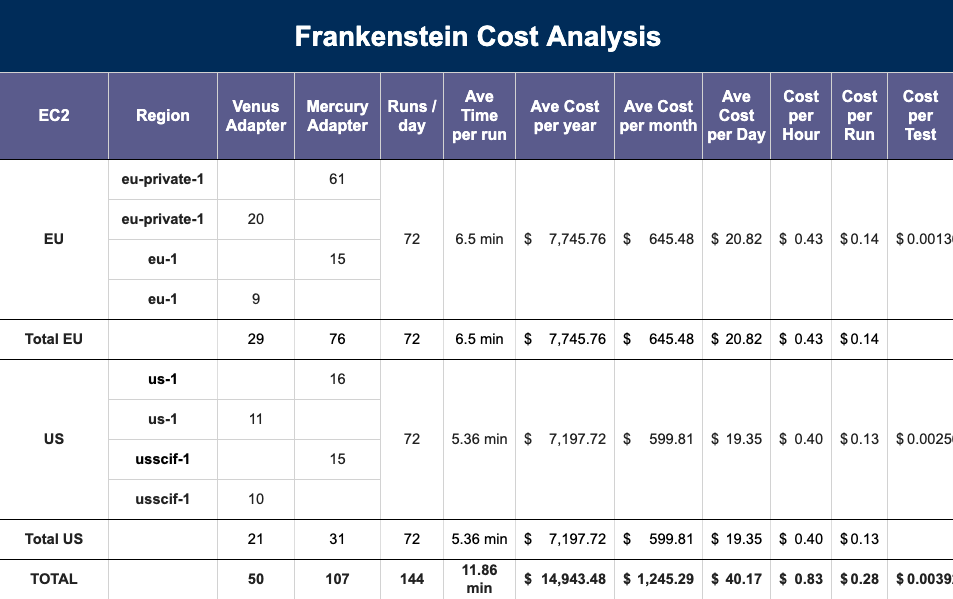
\includegraphics[width=\textwidth,height=\textheight,keepaspectratio]{./diagrams/frank_cost_analysis.png}
 \caption{Frankenstein Cost Analysis}
\end{figure}

\section{Research and Analysis of Possible Testing Frameworks for Bosco}

Frankenstein uses Mocha as its testing framework but there are multiple frameworks like Mocha. The following is an investigation into what else is available as well as a review of the current framework, Mocha.
\subsection{Mocha}

Mocha is a feature-rich JavaScript test framework running on Node.js and in the browser, simplifying asynchronous
testing. Mocha tests run serially, allowing for flexible and accurate reporting, while mapping uncaught
exceptions to the correct test cases. Mocha provides functions that execute in a specific order, logging the
results in the terminal window. Mocha also cleans the state of the software being tested to ensure that test
cases run independently of each other.

\begin{figure}[ht]
 \centering
 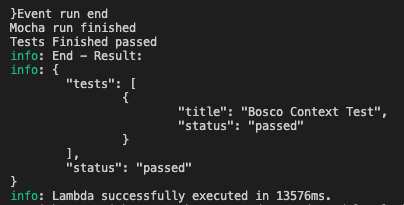
\includegraphics[width=\textwidth,height=\textheight,keepaspectratio]{./diagrams/mocha_test_result.png}
 \caption{Mocha Test Result Output}
\end{figure}

\subsection{Jest}

Jest is a JavaScript testing framework created by Facebook. It is open source, well-documented and popular due to its
high speed of test execution. It comes with a test runner, but also with its own assertion and mocking library unlike Mocha where you need to install an assertion
library, there is no need to install and integrate additional libraries to be able to mock, spy or make assertions.

\subsection{Mocha vs Jest}

\begin{table}[H]
 \centering
 \small
 \setlength\tabcolsep{6pt}
 \begin{tabular}{|c|c|c}
  \hline \textbf
  {Mocha}       & \textbf {Jest}\\
  \hline\hline
  Flexible configuration options & High Speed of Test Execution\\
  \hline
  Good Documentation       & Good Documentation\\
  \hline
  Ideal for back-end projects  & Test Runner included\\
  \hline
  Ad-hoc library choice     & Built in assertion and mocking library\\
  \hline
 \end{tabular}
 \caption{Mocha Vs Jest}
\label{table:mocha:jest}
\end{table}

\section{Review of Puppeteer}

Puppeteer is a popular test automation tool maintained by Google. It automates Chrome and Firefox and is relatively simple and stable to use.
Fundamentally Puppeteer is an automation tool and not a test tool.
This means it is incredibly popular for use cases such as web scraping, generating PDFs, etc.

Testing user flows within web applications usually involves either using an automated headful
browser (i.e. FireFox with Selenium) or a Headless browser, one that presents no UI, that is built on top of its own unique JavaScript
engine (i.e. Testcafe). This creates a situation where trade offs have to be made: speed vs. reliability.
Puppeteer aimed to remove this trade off – by enabling developers to leverage the Chromium browser environment
to run their tests and by giving them the flexibility to leverage headless or headful browsers that run on the same underlying platform as their users.

\subsection{Pros of using Puppeteer}

\begin{itemize}
 \item Simple to set up.
 \item Good documentation. Small community but lots of tutorials at this point.
 \item Promise based.
 \item Scriptable web browser
 \item Installs Chrome in a working version automatically
 \item Thin wrapper
 \item Bi-Directional (events) \- automating things like console logs is easy
 \item Maintained by Google.
 \item JavaScript first, so the code feels very natural
 \item Puppeteer also gives you direct access to the Chrome DevTools Protocol if you need it. Which can be very useful at times and in general it feels like there are fewer moving parts.
 \item Works with multiple tabs and frames. It has an intuitive API
 \item Trusted Actions: This criterion means dispatching events by the user agent which allows for user agent behaviours like hovers.
 \item End to end tests are very fast in practice but people suffer misconceptions regarding the execution speed. Typically, it’s the website or web-app that are slow and the tests end up waiting for the web app to be ready most of the time.
 \item Pro and Con: Stability which means how often tests fail after being authored other than when detecting a real application bug. Puppeteer wait for certain thing but has to waitFor manually for others.
 \item Debugging: Can write and debug Javascript from an IDE.
\end{itemize}

\subsection{Cons of using Puppeteer}
\begin{itemize}
 \item Limited cross-browser support—only Chrome and Firefox
 \item Feels like an automation framework and not a test framework—you often have to re-implement testing-related tools
 \item Grids (running concurrently) in production are often a challenge
 \item The automatic browser set up downloads Chromium and not Chrome and there are subtle differences between the two.
 \item Smarter Locators : No support for selecting elements in multiple ways
 \item Does not support parallelism, grids and infrastructure. Usually people build their own but this is due to change soon.
 \item Does not support self healing tests and automatically improving tests.
 \item Does not support Autonomous testing which is testing without code or user intervention.
\end{itemize}

\subsection{Testcafe Vs Puppeteer}

Puppeteer is a Node library which provides browser automation for chrome and chromium.
TestCafe is a Node.js tool to automate end-to-end web testing. Puppeteer runs headless by default,
but can be configured to run full (non-headless) Chrome or Chromium; It provides a high-level API to
control Chromium or Chrome over the DevTools Protocol. TestCafe runs on Windows, MacOs, and Linux and
supports mobile, remote and cloud browsers (UI or headless). It is also free and open source.

\clearpage

\begin{figure}{h}
 \centering
 \subfloat[\centering Npm Downloads]{{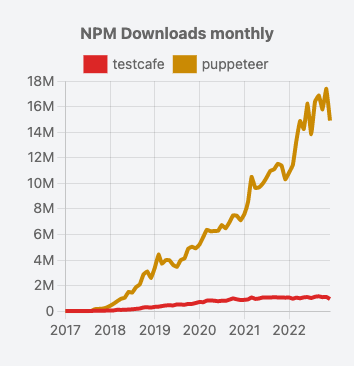
\includegraphics[width=5cm]{./diagrams/npm_pupp_tc}}}
 \qquad
 \subfloat[\centering GitHub stars]{{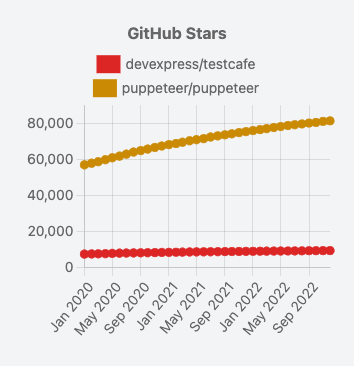
\includegraphics[width=5cm]{./diagrams/github_stars}}}
 \caption{NPM statistics}
\end{figure}

\section{EC2 vs Lambda comparison}

AWS Elastic Compute Cloud (EC2) is basically a virtual machine called an instance. Users can create an instance and define
the resources neccessary for the task at hand. For example the type and number of CPU, memory, local storage and scalability. EC2 instances
are intended for consistent, static operations and users pay a recurring monthly charge based on the size of the instance, the operating
system and the region. The instances run until they are deliberately stopped.

Lambda on the other hand is billed per exectution and per ms in use with the amount of memory the user allocates to the function.
When a lambda funciton is invoked, the code is run without the need to deploy or manage a VM. It is an event based service that is
designed to deliver extremely short-term compute capability. AWS handles the back-end provisioning, loading, execution, scaling and unloading of the user's code.
Lambdas only run when executed yet are always available. They scale dynamically in response to traffic.

\section{Conclusion}
// TODO

\chapter{Initial Design Implementation}

\section{Proof of Concept - Running Puppeteer on a Lambda}

In order to prove it is possible to run Puppeteer tests on AWS Lambda, a basic end to end test was designed
to run with Puppeteer. This automated a scenario whereby a browser, Chromium was launched with the url of the
messenger page. After the page loaded, the messenger button was toggled and the chatbot would load. The test
passed if the text from the messenger returned the expected output text.

\subsection{Mocha}

The mocha test framework was added to the code as in reality Puppeteer is not a test framework but an automation tool.
Assertions are made using the Assert library package and logged to the console but it is not in essence a testing tool.
Once mocha was configured and run without errors the next step was to run the script in a lambda.

\begin{figure}[h]
 \begin{tcolorbox}
  \begin{minted}[breaklines]{javascript}
  // simple-test.js
  const puppeteer = require("puppeteer");
  const url = process.argv[2];
  if (!url) {
    throw "Please provide URL as a first argument";
  }
  async function run () {
   const browser = await puppeteer.launch();
   const page = await browser.newPage();
   await page.goto(url);
   await page.screenshot({path: "screenshot.png"});
   browser.close();
  }
  run();
\end{minted}
\end{tcolorbox}
\captionof{figure}{Simple test written with Puppeteer}
\end{figure}

However, there are problems running Puppeteer in a lambda. Lambda has a 50 MB limit on the zip file you can upload. Due to the fact that it installs Chromium, the Puppeteer package is significantly larger than 50 MB\. This limit does not apply when uploaded from an S3 bucket but there are other issues. Linux including AWS Lambda does not include the necessary libraries required to allow Puppeteer to function.

\subsection{Node Modules}

There are work-arounds for this in the form of node modules, \'puppeteer-core\' and \'chrome-aws-lambda\'.
Both these modules installed allow for a version of Chromium that is built to run for AWS Lambda. Incorporating
these ensures the tests run successfully. Unfortunately these modules need to be in parody with each other.

The aws-chrome-lambda module has not been updated since June 2021 so its latest version is 10.1.0 whereas
puppeteer-core has been updated regularly and is at present at version 19.3.0. When the version numbers are
synced the lambda function passes. Obviously this is not ideal as there is a vast difference between versions.
Whatever the reason for these modules not being updated, relying on them is impractical and will eventually lead to our tests being broken.

\subsection{Docker}

The process uses a Docker container instead of node modules to condense the code. A Docker
container is a standalone piece of software that packages up code and all its dependencies so the application runs quickly and reliably from one computing environment to the next.
A Docker container image is a lightweight, standalone, executable package of software that includes everything needed to run an application: code, runtime, system tools, system libraries and settings.
Container images become containers at runtime. Containers isolate software from its environment and ensure that it works uniformly despite differences for instance between development and staging.

The puppeteer test runs locally using a Docker engine, then gets tagged and pushed to a container on a Lambda function named \'puppeteer-container\'.
This significantly speeds up the testing process, automating a browser in milliseconds compared to the previous method's average time of six seconds.
The process provides more control over the testing environment and successfully runs the tests by targeting a number of tests through event handler parameters instead of hard coding.
The results validate the feasibility of running tests in a Lambda using Puppeteer.

\subsection{Conclusion}

The process tests the use of Puppeteer and Mocha as an automation tool in a Lambda container and finds that deploying an image through Docker is a more reliable solution. The tests can be run locally with Docker and then uploaded to the Lambda container. The results are recorded in Cloudwatch logs for monitoring and assessment.

\section{Initial Stepfunction Research and Development}

One possible infrastructure that is important to explore is the use of of step functions for the test suite. With 
step functions a workflow can be created through a series of lambda functions with each step being a state within
the workflow. They are based on a state machine and tasks where a state machine is a workflow and a task is a
state in that workflow that another AWS service performs.

\begin{figure}[h]
 \centering
 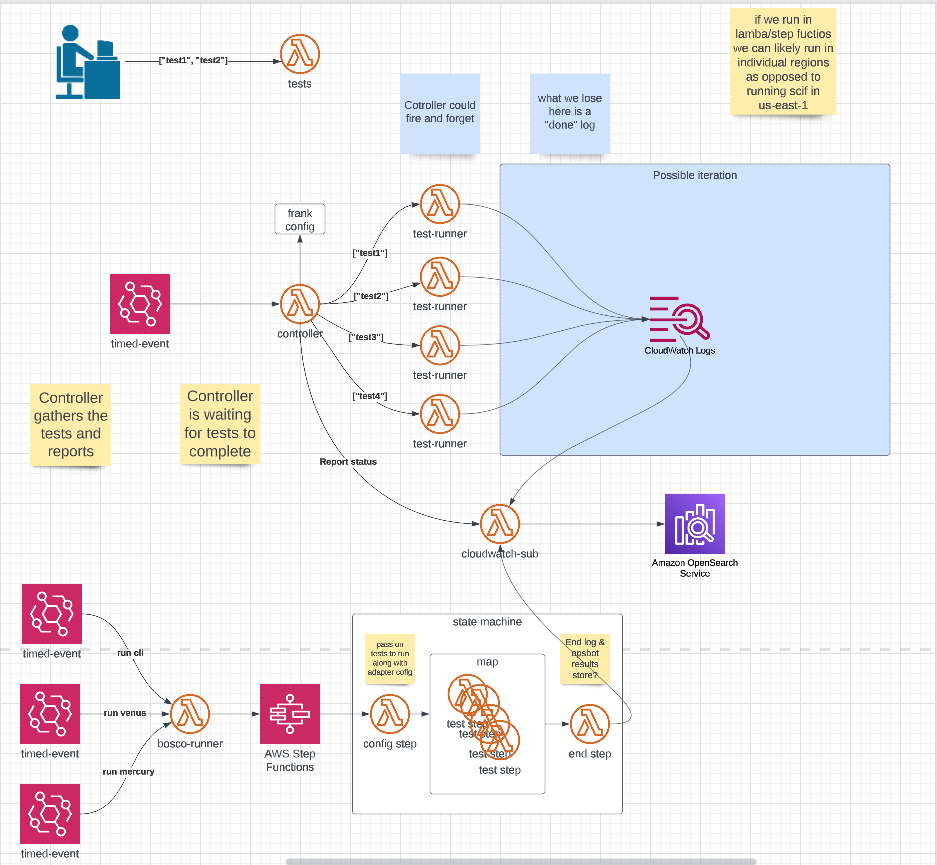
\includegraphics[width=15cm]{./diagrams/possible_implementation}
 \captionof{figure}{Bosco Planned Implementation}
\end{figure}

\section{State Transitions}

The Bosco test suite runs through 5 state transitions (Start, StartState, Map, Done, End) plus an additional transition for each test run (Running). With three tests, there are 8 states as the \"Running\" state is executed three times. The first state is the \"Start\" state which initiates the run and then the \"StartState\" is invoked, creating an array of tests and passing the payload to the \"Map\" state.

This experiment focuses on using the Inline Map state instead of the Distributed Map state. The Inline Map state is used for fewer than 40 parallel iterations while the Distributed Map state is used for larger workloads. The map state runs a lambda for each test, which runs in parallel with each other. The results of the tests are then outputted to the \"Done\" lambda, the next state, which processes and runs the tests. Finally, a state prints out the results and the End state completes the workflow.

\begin{figure}[h]
 \centering
 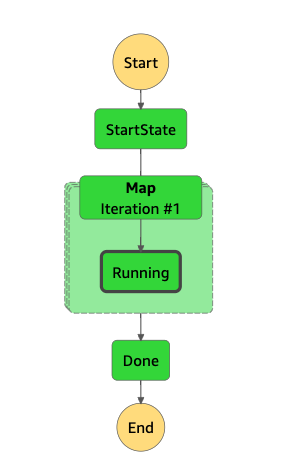
\includegraphics[width=5cm]{./diagrams/step_function}
 \caption{Bosco State Machine}
\end{figure}

\begin{figure}[h]
 \centering
 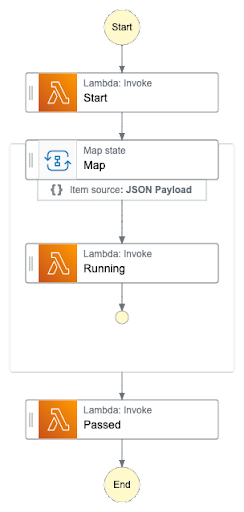
\includegraphics[width=5cm]{./diagrams/state_machine}
 \caption{Inline Map State for Bosco Step Function}
\end{figure}

\subsection{Cold vs Warm Lambdas}

Comparisons were made between running the tests on cold lambdas as opposed to warm lambdas and the results were significantly different. The cold lambda run ran in 40 seconds and the warm lambda run ran in 14 seconds total which is more than half the duration. Further investigation will take place when actual Frankenstein tests can be added to our state machine.

\subsection{Cost Analysis of Step Function State Machine}

The cost of running the test suite in a state machine using AWS Step Functions is based on the number of state transitions. This cost analysis does not account for error handling, which may increase the cost due to retries. The cost per transition is \$0.000025 according to the AWS pricing calculator. The analysis is based on the current number of tests and the frequency they are run (three times an hour), which may vary for Bosco tests.

\begin{figure}[h]
 \centering
 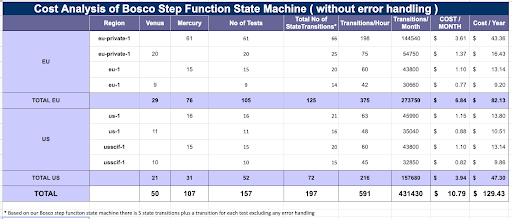
\includegraphics[width=15cm]{./diagrams/sf_cost_analysis}
 \caption{Bosco Step Function Cost Analysis}
\end{figure}

\chapter{Bosco Implementation}

\section{Lightning Page}
The implementation of Bosco has begun after finalizing the proof of concept. The first step involves refactoring the Frankenstein Lightning page, which serves as the source for all selectors and functions related to the Messenger page. To avoid duplication, a constructor was created and a function was added to launch the browser and open the Messenger page.

\begin{figure}[H]
 \begin{tcolorbox}
  \begin{minted}{js}
 async goToPage() {
  await this.page.goto(this.url, 
  { waitUntil: 'networkidle2' });
 }
\end{minted}
 \end{tcolorbox}
 \caption{Example of a Lightning function}
\end{figure}

With this starting point the interaction node test was refactored to use the Lightning page. Two functions were
created, one which clicks through the selectable list and another function which types into messenger instead of
clicking the list. A BrowserFactory class was created which has a function to create the browser.

\section{Developer Dependencies}
\textbf{ESLint} was also added to the project which is a linting tool that ensures all the code is formatted consistently
by anyone who makes changes to the code.  

\textbf{loglevel} was added to replace the console.logs and a dependency check
was added which checks for unused dependencies before commits.  Once the test was running without errors the work
was committed, the code reviewed and the POC branch was merged into the master branch on the Bosco repository.

\textbf{lambda-local}, a node module was used for testing purposes. This allowed for the running of the lamdas locally rather than having 
to deploy each time they were to be tested. 

\section{Context Test}
The first actual Frankenstein test to be converted to Bosco was the Context test. This test sets the context from the url
and tests if it is outputted with the rest of the context.  This was interesting to work on as it exposed a bug in the Frankenstein test had a bug in it so it was not testing what it was supposed to be
testing even though the test was passing. Once the error was highlighted I was able to finish writing the test
and ensure it was working correctly. I made a PR, Dean reviewed it. I made the changes Dean suggested which
included tidying up the code.

\section{Conversation Engaged Test}
The next task at hand is to convert the Conversation Engaged test. Whenever a user interacts with a bot, a goal is generated, which is a default or custom event that's tracked to measure the success of the bot's interactions.
At first, it was believed that this test would be simple, but changes were requested after a pull request was submitted for review, including removing nested if statements and improving the code's formatting.

This created a need to parse the exported goal JSON result. However, an error was encountered in the Servisbot CLI proxy, where the outputted JSON was not formatted correctly and could not be parsed. To work around this, the CSV output option was used instead of JSON and the csv-parse node module was imported.
To test this, a temporary script named \"proxy.mjs\" was created to run the goals part of the test independently. It was discovered that csv-parse/sync needed to be imported instead of just csv-parse and that VSCode needed to be restarted as it was not running the code. After discussing the issue with colleagues and having them run the code on their machines, it was concluded that the problem was with VSCode and simply restarting it solved the issue.

\section{Cloud Formation}
The Bosco project will be deployed using Cloud Formation, a deployment tool.
The Cloud Formation template, which can be in either yaml or json format, specifies the necessary environment variables and resources.
The aim is to upload the start, done, and test runner lambda functions through Cloud Formation and have the state machine reference these lambdas.
Once this is complete, the state machine will invoke the lambdas.

The cloud formation template will have three lambda functions.
The start function, the test runner which points to the image of the container and the done function. The
template will also contain the state machine definition. A YAML formatting extension from Redhat to format the YAML
file is also necessary as it is not possible to deploy the YAML unless the format is accurate.

To log into the ServisBOT cli a \.env file containing authentication details can be added as a temporary solution.
The environment variables will be read through AWS SSM eventually.

\section{Environment Variables}
The next objective is to supply the handler with the environment variables through the orchestration lambda.
The final result is to have an array called TestSuite, consisting of elements, each of which contains two arrays: one for tests and the other for environment variables.
The tests array can contain either a single test or an array of tests, but it is structured in a way that each element in the TestSuite array is also an array,
which leaves room for running multiple tests in one lambda or running each test separately in different lambda functions.

Once it is possible to provide the environment variables to the handler via the orchestration lambda via an
object containing the test file path and the environment variables the next step is to provide a shared environment
between all lambda functions in the map. This can be achieved by providing the environment variables to the handler
at the same level as the array of tests and refactoring the state machine to use the environment variables for
each test. This was necessary to implement as environments can grow and therefore can be resource heavy on the
state machine. By providing one instance of environment variables rather than 40 test objects containing
environment variables and a test file path.

It is essential at this stage to ensure it is possible to flip between environments by either providing the JSON through the
orchestrator lambda function or by providing it to the State machine initiation step. If the JSON is provided by both, then the tests should run twice.

By providing the state machine with the environment variables and testSuite there is more control over the state
machine. What tests are run with what environment variables can be determined at any stage.

\section{Refactor of State Machine to use a Shared Environment on Individual Test Instances }

The state machine was then refactored to use a shared environment instead of
passing the environment variables in with each test object. In the state machine definition there is an option to
use an ItemSelector which allows the map to iterate over the ItemsPath but use the ItemSelector to add additional
parameters.

The updated definition of the state machine included the following extra parameters:

\begin{figure}[H]
 \begin{tcolorbox}
  \begin{minted}{json}

 "Next": "Done",
 "ItemsPath": "\$.testSuite",
 "ItemSelector": {
  "testSuite.\$": "\$\$.Map.Item.Value",
  "environment.\$": "\$.environment",
  "profile.\$": "\$.profile",
  "testConfig.\$": "\$.testConfig"

}
\end{minted}
 \end{tcolorbox}
 \caption{Definition of Map State including Test Profile}
\end{figure}

The input to the map state became the following:

\begin{figure}[H]
 \begin{tcolorbox}
  \begin{minted}{json}
{
 "tests": [
  {
   "path": "goals/puppeteer-conversation-engaged.js"
  }
 ]
}
\end{minted}
 \end{tcolorbox}
 \caption{Input to one Iteration of Map State with just the Test Path}
\end{figure}

In addition the input to each iteration of the running state became the following:

\begin{figure}[H]
 \begin{tcolorbox}
  \begin{minted}{json}
{
 "testConfig": {
  "endpoint": {
   "create": {
    "AutoFailover": true
   }
  }
 },
 "environment": [
  {
   "name": "ORGANIZATION",
   "value": "some-organization"
  },
  {
   "name": "USERNAME",
   "value": "some-username"
  },
  {
   "name": "PASSWORD",
   "value": "some-password"
  },
  {
   "name": "SERVISBOT_REGION",
   "value": "eu-private-3"
  },
  {
   "name": "LOG_LEVEL",
   "value": "INFO"
  }
 ],
 "testSuite": {
  "tests": [
   {
    "path": "goals/puppeteer-conversation-engaged.js"
   }
  ]
 },
 "profile": "eu-private-3-venus"
}

\end{minted}
 \end{tcolorbox}
 \caption{Running State Input including Shared Environment}
\end{figure}

\section{Test Profiles}
One significant way in which Bosco will differ to Frankenstein is in the capability to run test profiles rather than 
running all the tests, all the time, in all the regions. By creating a test profile it is possible to specify which 
environment, region and frequency of the tests which Frankenstein does not have the ability to do. 

A profiles folder was created with two different profiles for the adapters Venus and Mercury in the dev environment. Each profile 
contained the test suite so the orchestrator needed to be updated in order to read the file paths from the JSON provided in the 
event profile. The node module \textbf{file system\&(fs)} was used to read the contents of the profile, this was parsed to 
a javascript object and a spreader operator was used to combine the contents of the profile and the contents of 
the even inputted to the orchestrator and output these to the handler.

\begin{figure}[H]
 \begin{tcolorbox}
  \begin{minted}[breaklines]{javascript}
  const readProfile = fs.readFileSync(testProfile, (err, data) => {
  if (err) throw err;
   logger.info(data);
  });
  const profile = JSON.parse(readProfile);
  const output = { ...profile, ...event };
  \end{minted}
 \end{tcolorbox}
 \caption{Parsing a JSON string to a javascript object and use of the spreader (\dots) operator}
\end{figure}

Next the global environment variables were removed so instead of reading them from the input to the orchestrator they would 
be passed from the profile to the tests. There was quite a lot of code build needed for this as Mocha is limiting in that it doesn't 
allow the passing of parameters to the tests. 

\subsection{Singleton Class: TestRunnerConfig}
A singleton class was created to overcome this. A siingleton class is a class that can only have one instance of 
itself. It is used when there is going to be no change or update to the object for the duration it is used. This would be the case with our tests as we would just be using the configuration for accessing the lightning page to run the tests.

Initially the TestRunnerConfig took in the runnerEvent and created an instance of itself. It had getters to get different variables from the event which at the time were just the profile, testConfig, testSuite and environment. The tests ran but now the aim was to remove process.env to set the variables and use an Environment class that instead reads the environment variables from the TestRunnerConfig.

An Environment object was created using the environment from the event. This could now be accessed in the tests by calling the getters from the Environment object.
\begin{figure}[H]
 \begin{tcolorbox}
  \begin{minted}[breaklines]{javascript}
const testRunnerConfig = TestRunnerConfig.getInstance();
const environment = testRunnerConfig.getEnvironment();
const params = {
organization: environment.getOrganization(),
username: environment.getUsername(),
password: environment.getPassword(),
region: environment.getSBRegion()
};
\end{minted}
 \end{tcolorbox}
 \caption{Replacing proccess.env with getters to an Environment class invoked by a singleton class, TestRunnerConfig}
\end{figure}

\section{Endpoint Proxy}

Bosco needed to support both Mercury and Venus engagement adapters similar to Frankenstein. This is achieved through the endpoints whereby 
each endpoint is suffixed by the test profile name. When the endpoint is created instead of creating it uniquely with the timestamp, middleware 
in the form of an Endpoint proxy would instead suffix the endpoint with the profile and thereby point the tests to the url 
containing the endpoint proxy. To prove the tests were making network calls to either Mercury or Venus, the tests were slowed down, run in headful mode and 
the network tab examined. When the browser was talking to Venus there calls to \textbf{VendAnonConversation} and \textbf{ReadyForConversation} and when there were calls to Mercury, \textbf{graphql} calls were evident.

\begin{figure}[h]
 \centering
 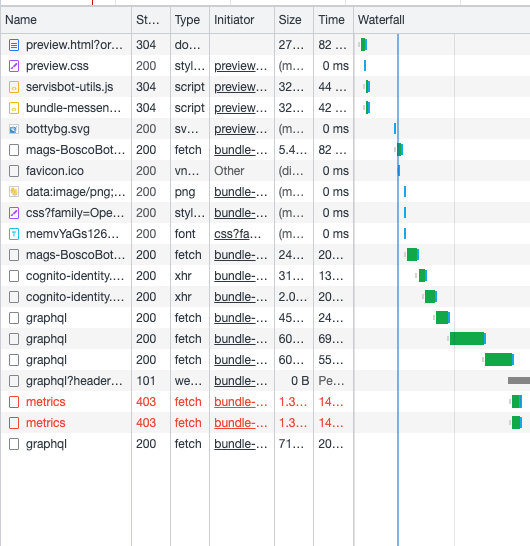
\includegraphics[width=15cm]{./diagrams/mercury_network_calls.png}
 \caption{Mercury Network Calls}
\end{figure}

\begin{figure}[ht]
 \centering
 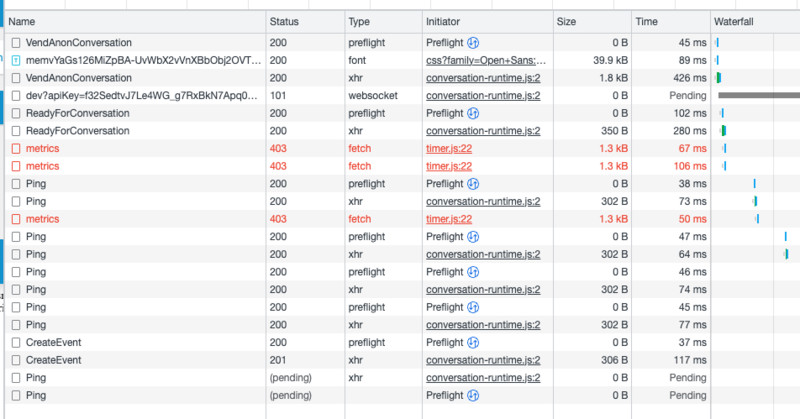
\includegraphics[width=15cm]{./diagrams/venus_network_calls.png}
 \caption{Venus Network Calls}
\end{figure}

\section{Creating a Test with a Secret}
Many of the Frankenstein tests use secrets in order to run the tests. Secrets can be defined as secure documents containing access keys, api keys, api secrets or IDs to external systems. They can be created and stored in the ServisBOT system and then referenced by bots securely. This is how ServisBOT manage API keys for AWS.

The test that was chosen was the NLP worker, Lex V2, intent-publish test. A \textbf{Lex} worker is a remotely managed NLP worker who takes input and sends it to a Lex bot for Natural Language Processing. A Lex bot is an Amazon bot, users use ServisBOT to access, manage and run their Lexbots. 
\textbf{NLP} is a form of Artificial Intelligence that transforms text that a user submits into language that the computer programme can understand. In order for ServisBOT to classify utterances using a remote managed NLP, the correct API keys, access tokens or cross account roles need to be configured in the ServisBOT Secrets Vault.

An AWS cross account role, ie a secret, is required in order to access Lex. An environment variable was created that the test could access called LEX\_V2\_CROSS\_ACCOUNT\_ROLE\_SECRET and to this was assigned the secret definition for dev in JSON format. 

This test creates a long living bot which is a bot that is not deleted after the test but is created the first time the test is run and then reused for every test. The bot's variable intent is updated with the timestamp every time to ensure the bot is publishing successfully. When the bot is publishing its status is polled every 5 seconds and when published its status is SUCCEEDED and so the test starts.

\begin{figure}[ht]
 \centering
 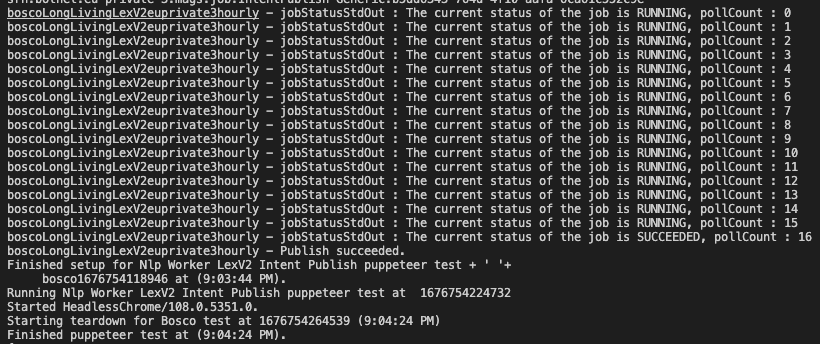
\includegraphics[width=15cm]{./diagrams/nlp_worker_poll.png}
 \caption{NLP worker test with polling}
\end{figure}

\section{SSM Parameters}
The next task for Bosco was to build the environment in the orchestrator using SSM parameters. 
SSM parameters are credentials and secrets that are stored in AWS Systems Manager parameter store. 
They can be encrypted and the service is easy and free to use. A few lines of code can retrieve the parameters from the store. 

The steps to this task were as follows:
\begin{itemize}
\item The parameters were created in the SSM parameter store in the same format as the Frankenstein parameters.
\item Code was added to the orchestrator to read the SSM parameters using the node module \textbf{aws-sdk}.
\item A new policy was added to the cloud formation template in order to give IAM permissions to read from the parameter store
\item The environment was built in the orchestrator by retrieving the ssm parameters in the orchestrator, building the envirnoment object and returning this to the output.
\item A new class, Secrets was added in order to retrieve the SSM parameters from the parameter store to extract that work from the orchestrator. Later to be renamed EnvironmentResolver. This was done by passing the ssm through to the Secrets constructor.
\item The README was updated to reflect the changes.
\end{itemize}

\begin{figure}[h]
 \centering
 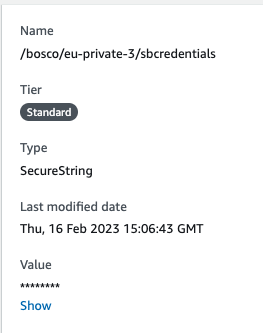
\includegraphics[width=8cm,height=8cm,keepaspectratio]{./diagrams/ssm_params.png}
 \caption{SSM Parameters created in AWS Systems Manager}
\end{figure}

\section{Eventbridge Rules (CRON) }

Like Frankenstein, Bosco needs to run on a scheduled event. WS Eventbridge allows developers to trigger evAents on a CRON which is `a command to an operating system or server for a job that is to be executed at a specified time`. 
To trigger the state macine to run different profiles at different times, in different regions the cloud formation file needed to be updates. 
\begin{itemize}
 \item First the rule defaults were added to the cloudformation
 \item The CRON rules were then added 
  \begin{tcolorbox}
   \begin{minted}[fontsize=\footnotesize, breaklines]{yaml}
   ScheduleMercuryExpression: { Type: String, Default: "cron(0,20,40 * * * ? *)" } # run at 0,20,40 past the hour
   ScheduleVenusExpression: { Type: String, Default: "cron(10,30,50 * * * ? *)" } # run at 10,30,50 past the hour
   ScheduleHourlyExpression: { Type: String, Default: "cron(0 * * * ? *)" } # run at 0 past the hour
   \end{minted}
  \end{tcolorbox}

 \item The triggers were added.
 \begin{tcolorbox}
  \begin{minted}[fontsize=\footnotesize, breaklines]{yaml}
   EuMercuryTriggerEnabled: !Equals [ !Ref MercuryEuRunnerEnabled, "true" ]
   EuVenusTriggerEnabled: !Equals [ !Ref VenusEuRunnerEnabled, "true" ]
   EuHourlyTriggerEnabled: !Equals [ !Ref HourlyEuRunnerEnabled, "true" ]
  \end{minted}
 \end{tcolorbox}
 \item The schedule rules were added
 \item A new Sceduled Event IAM role to execute the state machine was added with a special policy that allows the execution of the state machine. 
 
 \begin{tcolorbox}
  \begin{minted}[fontsize=\footnotesize, breaklines]{yaml}
    ScheduledEventIAMRole:
        Policies:
          - PolicyName: StateMachineExecutionPolicy
            PolicyDocument:
              Version: "2012-10-17"
              Statement:
                - Effect: "Allow"
                  Action: "states:StartExecution"
                  Resource:
                    - !Ref ImportBoscoStateMachine
  \end{minted}
 \end{tcolorbox}
\end{itemize}

\begin{figure}[h]
  \centering
  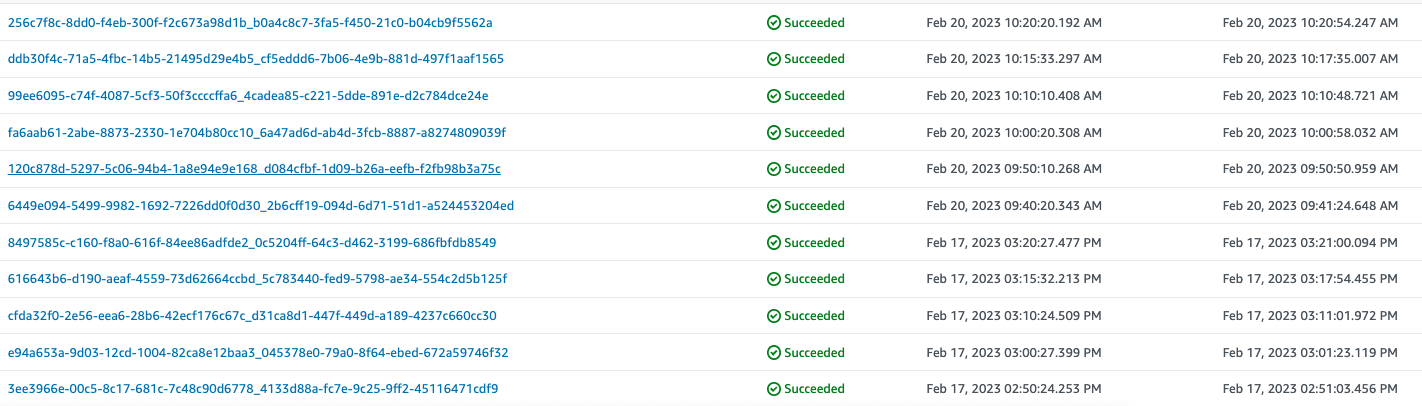
\includegraphics[width=15cm]{./diagrams/state_machine_cron_executions.png}
  \caption{R\&D Phase and Bosco Implementation Phase}
 \end{figure}

\appendix
\chapter{Methodology}
Jira was used to keep track the sprints on the Bosco project. Week long sprints were the chosen method for the implementation phase as this
was better suited to the type of project as the urgency to have it complete is high.

Once the cloud formation file was deployed successfully, it was possible to observe the timed events executing successfully. You can see from the following table 
that each execution is now given a unique ID and runs at regular intervals past the hour. The working CRON instigated time machine was showcased to the team and they were 
queried on whether they would liked the introdcution of a profile that ran hourly as opposed to every twenty minutes. The team agreed that the tests were already running too 
frequently and costing a lot. Bosco will have more control over what tests are run, in what regions and how frequently through the test profiles, therefore giving ServisBOT 
much more control over their testing suite and providing flexibility and control that Frankenstein seriously lacks in.

The projcet was broken into three Epics:

\begin{itemize}
  \item Bosco Research and Dessign
  \item Bosco Implementation
  \item Bosco Dissemination Phase
\end{itemize}
\section{Research and Design}\subsection*{0.1.0}
Research and Design was carried out over a number of weeks starting in December with the main focus on the following:
\begin{itemize}
\item Review Puppeteer
\item Review Lambda
\item Initial Step Function R\&D
\item Cost Analysis
\item Proof of Concept
\end{itemize}

\section{Implementation}\subsection*{0.2.0}
The implementation of Bosco was carried out in one week sprints as was required by the project supervisor in ServisBOT. 
\subsection*{0.2.1}
\begin{itemize}
\item Add two Frankenstein tests to Bosco
\item Step Function Lambda code moved to Bosco
\end{itemize}

\subsection*{0.2.2}
\begin{itemize}
\item Cloudformation
\end{itemize}

\subsection*{0.2.3}
\begin{itemize}
\item Bosco environment variables for tests
\item Refactor state machine to use a shared environment
\end{itemize}

\subsection*{0.2.4}
\begin{itemize}
\item Test profiles and overrides
\end{itemize}

\subsection*{0.2.5}
\begin{itemize}
\item Create a test with a secret
\end{itemize}

\begin{figure}[h]
 \centering
 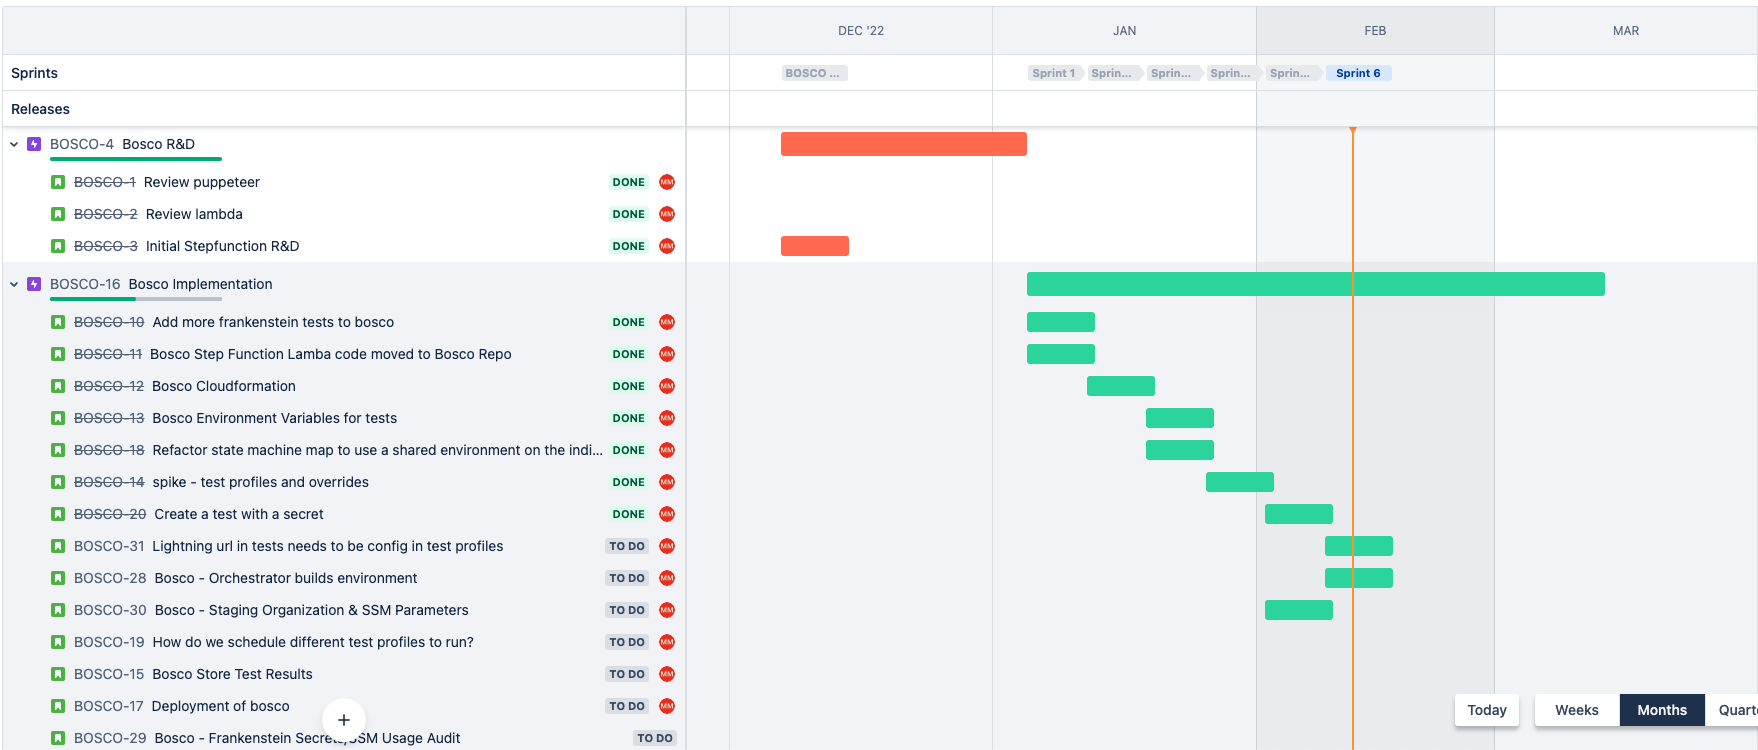
\includegraphics[width=15cm]{./diagrams/sprints1.png}
 \caption{R\&D Phase and Bosco Implementation Phase}
\end{figure}

\begin{figure}[h]
 \centering
 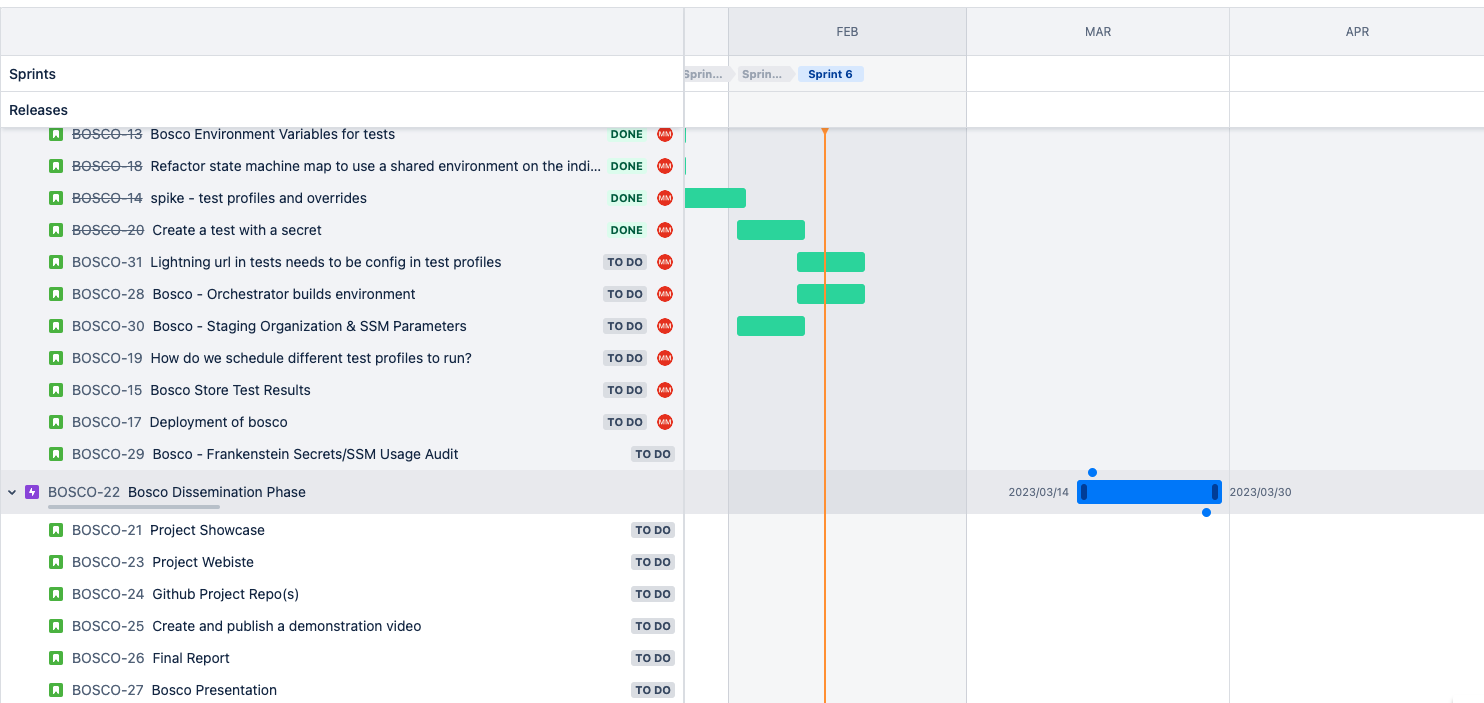
\includegraphics[width=15cm]{./diagrams/sprints2.png}
 \caption{Bosco Dissemination Phase}
\end{figure}


\chapter{Bibliography}

As \textcite{Jetty} says.

%No cite prints all references even if they are not in the document!!
% \nocite{*}
\printbibliography


% https://www.opsramp.com/guides/aws-monitoring-tool/cloudwatch-synthetics/
% https://www.functionize.com/automated-testing/assertion
% https://jestjs.io
% https://www.browserstack.com/guide/unit-testing-for-nodejs-using-mocha-and-chai
% https://www.tricentis.com/blog/bdd-behavior-driven-development
% https://www.pluralsight.com/blog/software-development/tdd-vs-bdd
% https://www.testim.io/blog/puppeteer-selenium-playwright-cypress-how-to-choose/
% https://www.testim.io/blog/webinar-summary-is-ai-taking-over-front-end-testing/
% https://aws.amazon.com/blogs/architecture/field-notes-scaling-browser-automation-with-puppeteer-on-aws-lambda-with-container-image-support/
% https://moiva.io/
% https://docs.aws.amazon.com/AmazonCloudWatch/
% https://docs.aws.amazon.com/lambda/latest/dg/gettingstarted-limits.html
% https://oxylabs.io/blog/puppeteer-on-aws-lambda
% https://aws.amazon.com/blogs/aws/new-for-aws-lambda-container-image-support/
% https://www.npmjs.com/package/chrome-aws-lambda
% https://www.docker.com/resources/what-container/
% https://blog.logrocket.com/testing-node-js-mocha-chai/
% https://www.ponicode.com/shift-left/
% https://blog.shikisoft.com/3-ways-to-schedule-aws-lambda-and-step-functions-state-machines/
% https://evanhalley.dev/post/aws-ssm-node/

\chapter{References}
//TODO
\end{document}